\begin{problem}[10]{Machine Learning: Overfitting}
Suppose we are doing parameter estimation for a Bayes' net, and have a training set and a test set. We learn the model parameters (probabilities) from the training set and consider how the model applies to the test set. In this question, we will look at how the average log likelihood of the training dataset and the test dataset varies as a function of the number of samples in the training dataset.

\begin{tabular}{@{}l@{}l@{}}
\begin{minipage}{0.75\textwidth}
Consider the Bayes' net shown on the right. Let $x_{1} \dots
x_{m}$ be the $m$ training samples, and $x'_{1} \ldots x'_{n}$
be the $n$ test samples, where $x_i = (a_i, b_i)$.
Recall that once we have estimated the required
model parameters (conditional probability tables) from the training data, the likelihood $L$
for any point $x_i$ is given by:
$$L(x_i) = P\left(x_i\right) = P(a_i)P(b_i|a_i) $$
We additionally define the \emph{log-likelihood} of the point $x_i$, to be $LL(x_i) = \log(L(x_i))$.
\end{minipage} &
\begin{minipage}{0.25\textwidth}
\begin{figure}[H]
\centering
    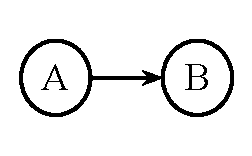
\includegraphics[width=1.0\textwidth]{figures/ml-tr-bayesnet.pdf}
\end{figure}
\end{minipage}\\
\end{tabular}


We use the log likelihood for a single point to define the average log likelihood on the training set ($\mbox{LL-Train}$) and the test set ($\mbox{LL-Test}$) as follows:
$$ \text{LL-Train} = \frac{1}{m}\sum_{i=1}^{m} LL(x_{i}) = \frac{1}{m}\sum_{i=1}^{m} \log\left(L(x_{i})\right) = \frac{1}{m}\sum_{i=1}^{m}\log\left(P(a_{i})P(b_{i}|a_{i})\right) $$
$$ \text{LL-Test} = \frac{1}{n}\sum_{i=1}^{n} LL(x'_{i}) = \frac{1}{n}\sum_{i=1}^{n} \log\left(L(x'_{i})\right) = \frac{1}{n}\sum_{i=1}^{n}\log\left(P(a'_{i})P(b'_{i}|a'_{i})\right) $$

We assume the test set is very large and fixed, and we will study what happens as the training set grows.

Consider the following graphs depicting the average log likelihood on the Y-axis and the number of training examples on the X-axis.
\vspace{-0.5cm}
\begin{figure}[H]
\subfloat[A]{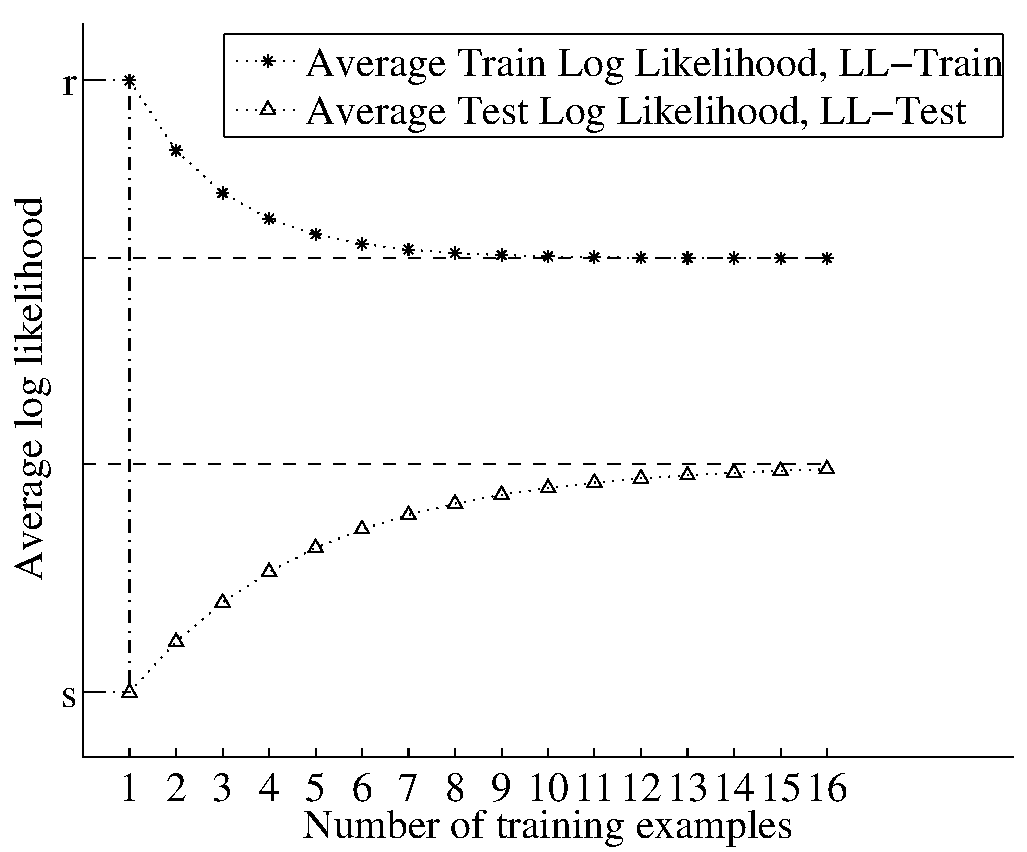
\includegraphics[width=0.25\textwidth]{figures/overfitting3.pdf}} \hfill
\subfloat[B]{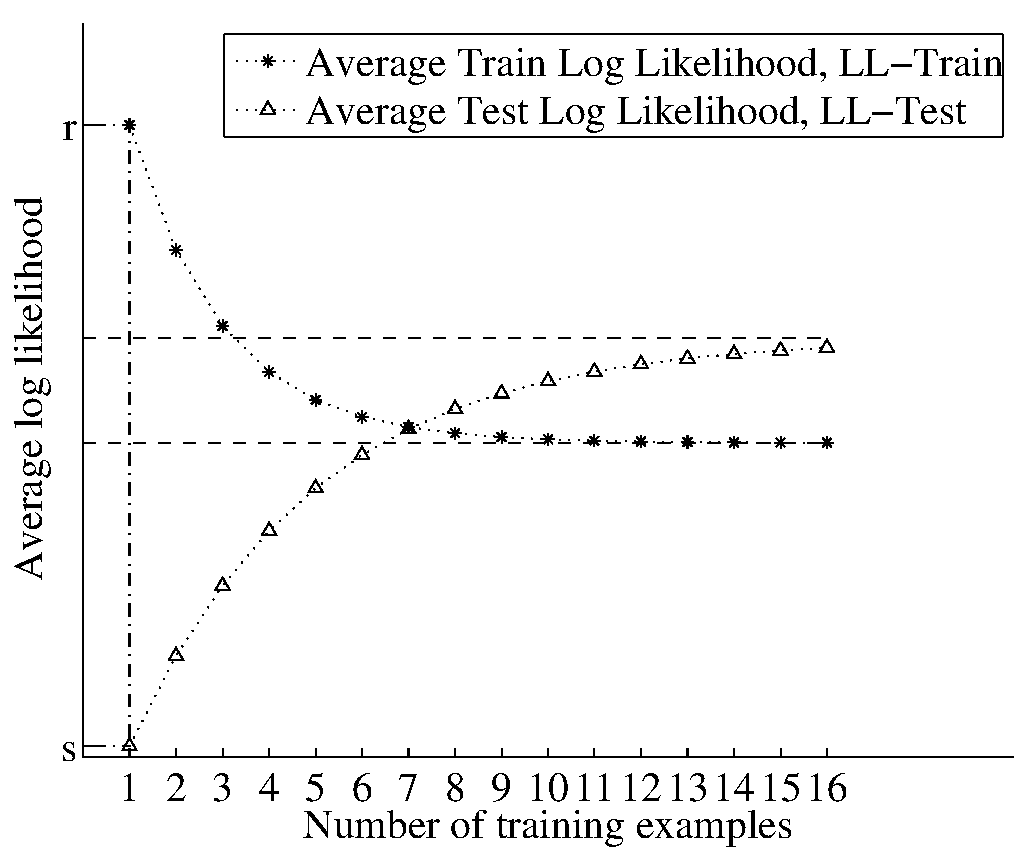
\includegraphics[width=0.25\textwidth]{figures/overfitting2.pdf}} \hfill
\centering \subfloat[C]{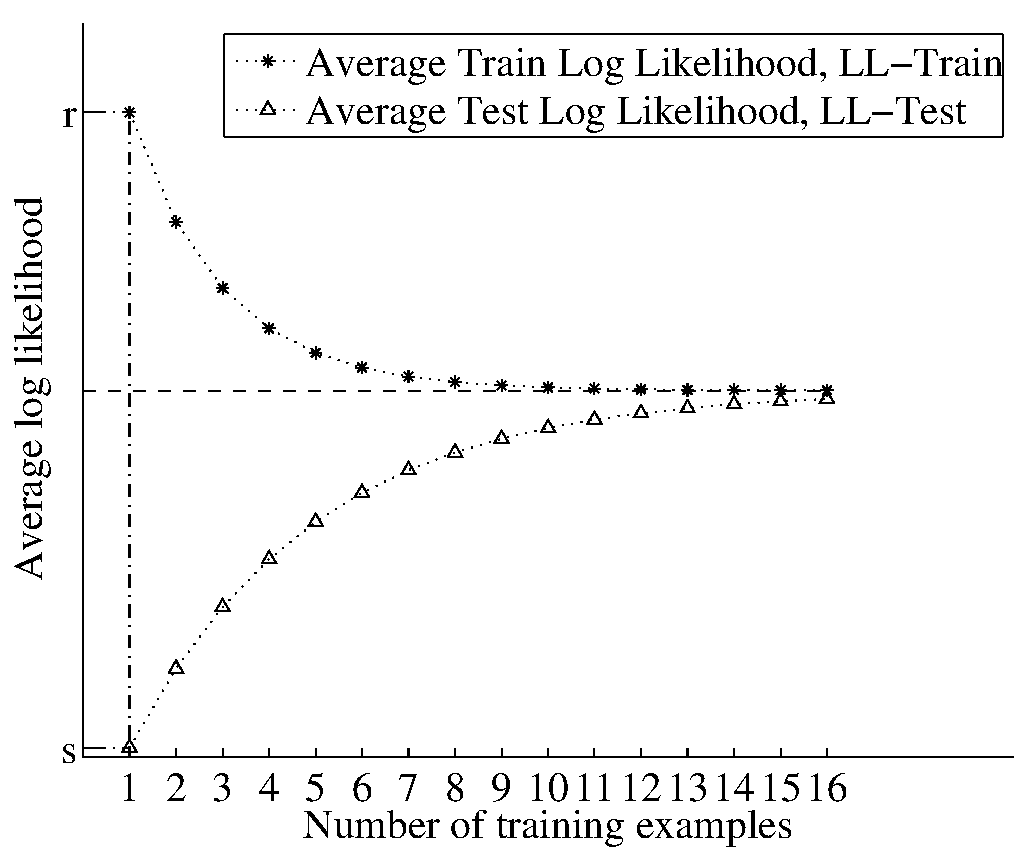
\includegraphics[width=0.25\textwidth]{figures/overfitting1.pdf}} \hfill \\
\subfloat[D]{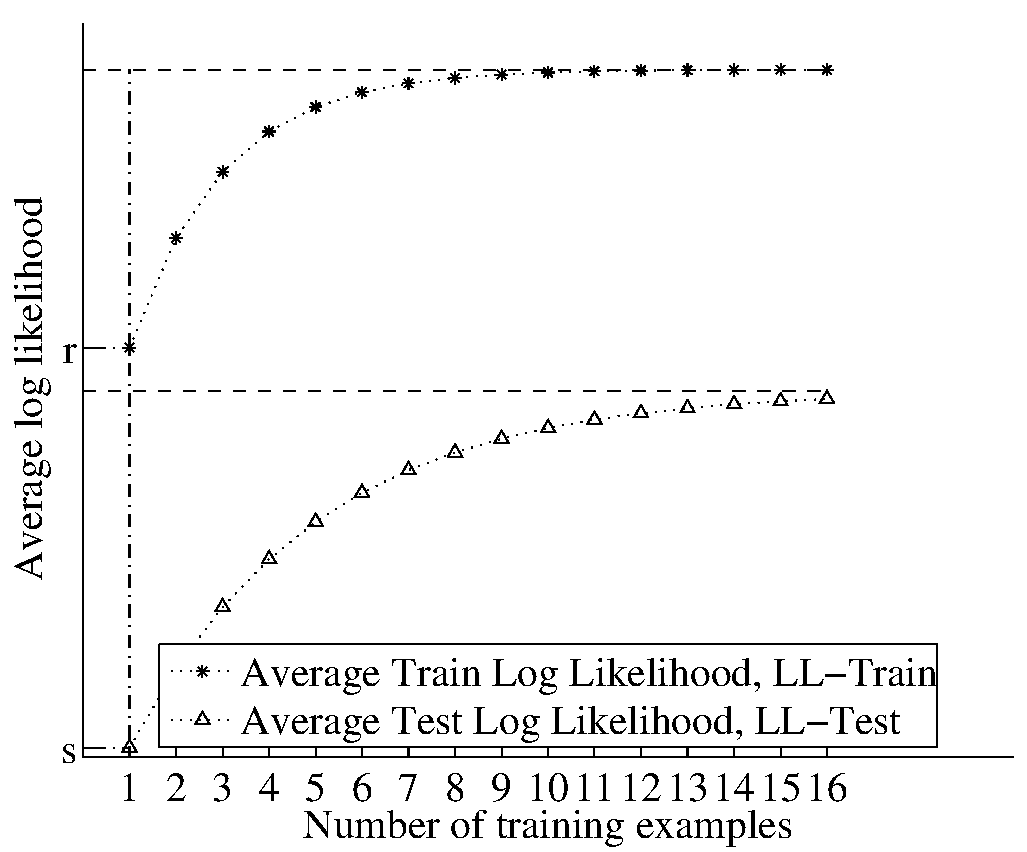
\includegraphics[width=0.25\textwidth]{figures/overfitting4.pdf}} \hfill
\subfloat[E]{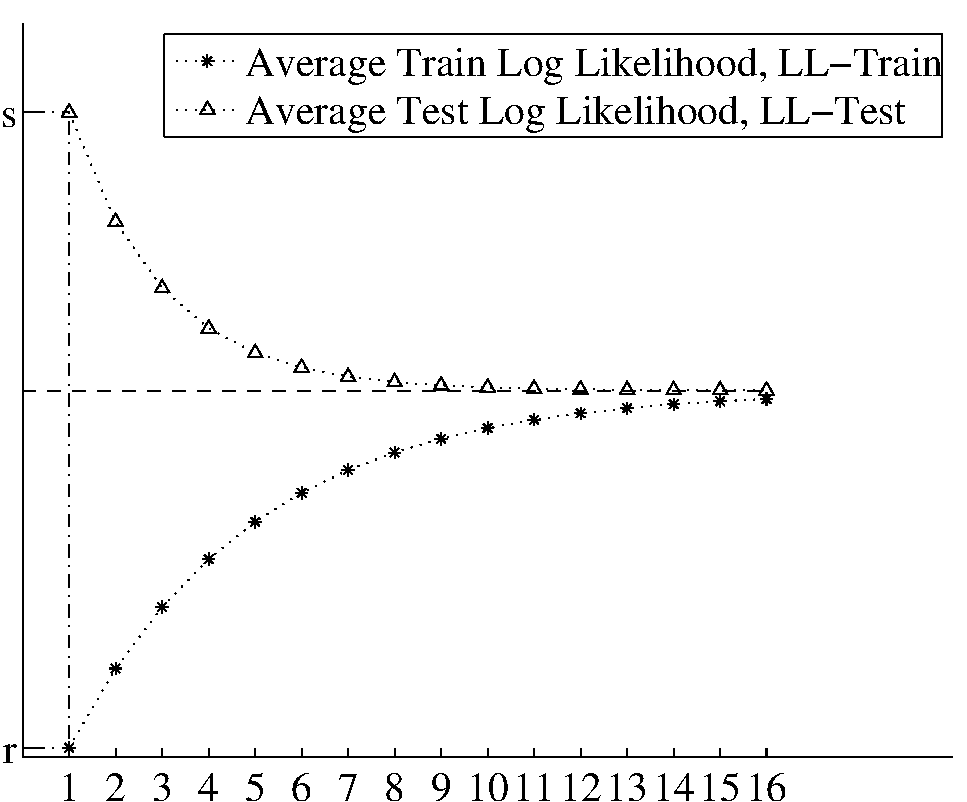
\includegraphics[width=0.25\textwidth]{figures/overfitting6.pdf}} \hfill
\centering \subfloat[F]{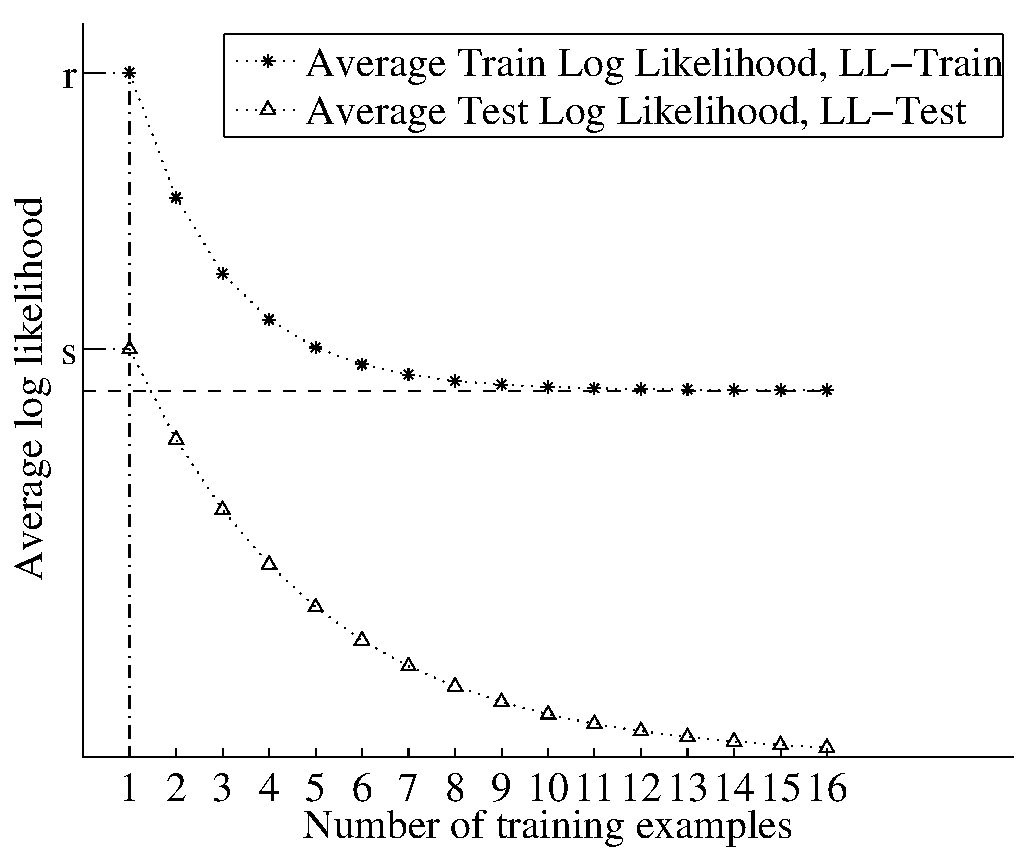
\includegraphics[width=0.25\textwidth]{figures/overfitting5.pdf}} \hfill \\
\end{figure}

\vspace{-0.3cm}
\begin{question}[2] Which graph most accurately represents the typical behaviour of the average log likelihood of the training and the testing data as a function of the number of training examples?
\begin{multicols}{6}
\begin{itemize}[label=, itemsep=12pt, topsep=12pt]
\OneA
\end{itemize}
\end{multicols}

\end{question}
\newpage
\begin{question}[2]
Suppose our dataset contains exactly one training example. What is the value of LL-Train?

\begin{multicols}{5}

\OneB

\end{multicols}

\end{question}

\begin{question}[3]
If we did Laplace Smoothing with $k=5$, how would the values of LL-Train and LL-Test change in the limit of infinite training data? Mark all that are correct. Briefly justify your answer.
\begin{multicols}{2}
\begin{itemize}[label=, itemsep=12pt, topsep=12pt]
\OneC
\end{itemize}
\end{multicols}
\solution{\vspace{0.5in}}{
   \fbox{\begin{minipage}[t][1.0cm][t]{18cm} 1c Explanation: \OneCExplanation \end{minipage}}\\
}
\end{question}

\begin{question}[3]
Consider the following increasingly complex Bayes' nets: $G_1$, $G_2$, and $G_3$.
\begin{center}
\vspace{-0.3cm}
\begin{tabular}{ccc}
$\qquad$
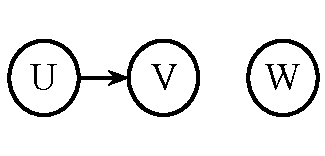
\includegraphics[width=0.20\textwidth]{figures/ml-overfitting-bn-1.pdf} $\qquad$ &
$\qquad$
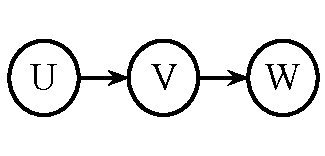
\includegraphics[width=0.20\textwidth]{figures/ml-overfitting-bn-2.pdf} $\qquad$ &
$\qquad$
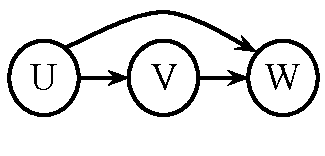
\includegraphics[width=0.20\textwidth]{figures/ml-overfitting-bn-3.pdf} $\qquad$ \\
$G_1$ & $G_2$ & $G_3$
\end{tabular}
\end{center}

Consider the following graphs which plot the test likelihood on the Y-axis for each of the Bayes' nets $G_1$, $G_2$, and $G_3$

\begin{figure}[H]
\centering
    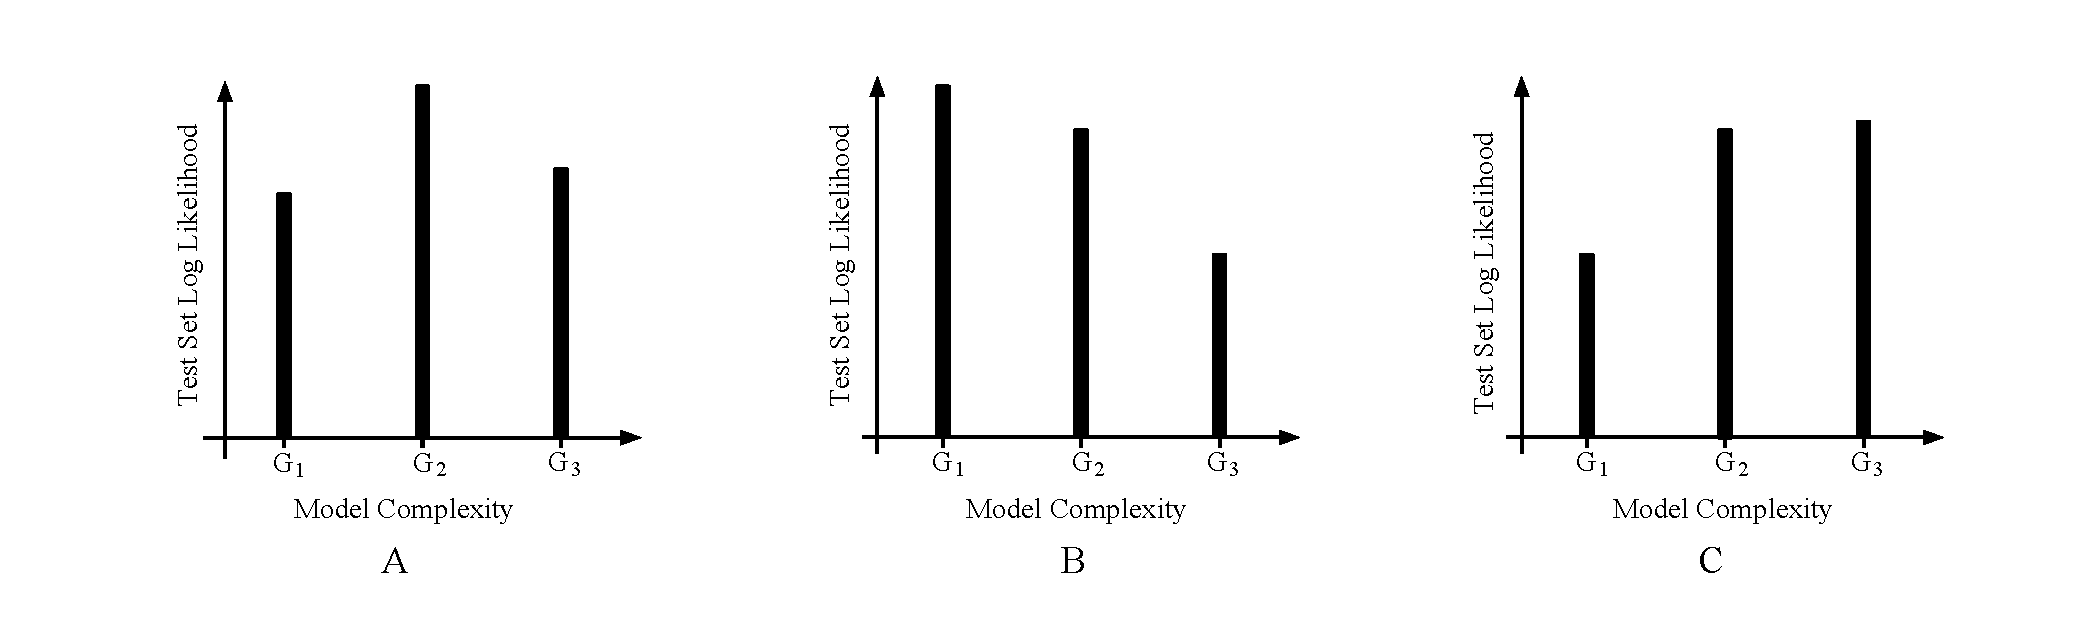
\includegraphics[width=1.0\textwidth]{figures/ml-overfitting-graphs.pdf}
\end{figure}
\vspace{-0.9cm}
For each scenario in the column on the left, select the graph that best matches the scenario. Pick each graph exactly once.
Briefly justify your answer.
\OneD \\
\solution{\vspace{0.5in}}{
   \fbox{\begin{minipage}[t][1.0cm][t]{18cm} 1d Explanation: \OneDExplanation \end{minipage}}\\
}
\end{question}
\end{problem}